\documentclass[10pt]{article}
\usepackage{pgfplots}
\pgfplotsset{compat=1.15}
\usepackage{mathrsfs}
\usetikzlibrary{arrows}
\pagestyle{empty}
\newcommand{\degre}{\ensuremath{^\circ}}
\begin{document}
\definecolor{qqwuqq}{rgb}{0,0.39215686274509803,0}
\definecolor{uuuuuu}{rgb}{0.26666666666666666,0.26666666666666666,0.26666666666666666}
\definecolor{zzttqq}{rgb}{0.6,0.2,0}
\definecolor{ududff}{rgb}{0.30196078431372547,0.30196078431372547,1}
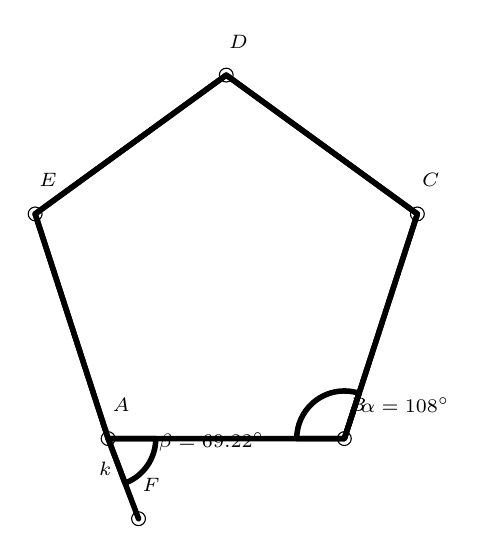
\begin{tikzpicture}[line cap=round,line join=round,>=triangle 45,x=1cm,y=1cm]

\draw [line width=2pt,fill opacity=0.10000000149011612] (-2,2) -- (1,2) -- (1.9270509831248424,4.85316954888546) -- (-0.5,6.61652530576288) -- (-2.927050983124842,4.853169548885461) -- cycle;
\draw [shift={(1,2)},line width=2pt,fill opacity=0.10000000149011612] (0,0) -- (72:0.6048542504621391) arc (72:180:0.6048542504621391) -- cycle;
\draw [shift={(-2,2)},line width=2pt,fill opacity=0.10000000149011612] (0,0) -- (-69.2245017165276:0.6048542504621391) arc (-69.2245017165276:0:0.6048542504621391) -- cycle;
\draw [line width=2pt] (-2,2)-- (1,2);
\draw [line width=2pt] (1,2)-- (1.9270509831248424,4.85316954888546);
\draw [line width=2pt] (1.9270509831248424,4.85316954888546)-- (-0.5,6.61652530576288);
\draw [line width=2pt] (-0.5,6.61652530576288)-- (-2.927050983124842,4.853169548885461);
\draw [line width=2pt] (-2.927050983124842,4.853169548885461)-- (-2,2);
\draw [line width=2pt] (-2,2)-- (-1.6140255659922953,0.9826047330006348);
\begin{scriptsize}
\draw  (-2,2) circle (2.5pt);
\draw (-1.8358054578284129,2.424174029935399) node {$A$};
\draw  (1,2) circle (2.5pt);
\draw (1.168303986133545,2.424174029935399) node {$B$};
\draw  (1.9270509831248424,4.85316954888546) circle (2.5pt);
\draw (2.0957471701754913,5.2871508154561875) node {$C$};
\draw  (-0.5,6.61652530576288) circle (2.5pt);
\draw (-0.34383164002180305,7.04122814179639) node {$D$};
\draw  (-2.927050983124842,4.853169548885461) circle (2.5pt);
\draw (-2.76324864187036,5.2871508154561875) node {$E$};
\draw (1.773158236595684,2.424174029935399) node {$\alpha = 108\textrm{\degre}$};
\draw  (-1.6140255659922953,0.9826047330006348) circle (2.5pt);
\draw (-1.4527310992023914,1.4160836124985008) node {$F$};
\draw[color=black] (-2.037423541315793,1.6177016959858803) node {$k$};
\draw (-0.6865823819503487,1.9604524379144257) node {$\beta = 69.22\textrm{\degre}$};
\end{scriptsize}

\end{tikzpicture}
\end{document}